\documentclass[border=10pt]{standalone}
\usepackage[utf8]{inputenc}
\usepackage{tikz}
\usetikzlibrary{shapes.geometric, arrows.meta, positioning}

\begin{document}

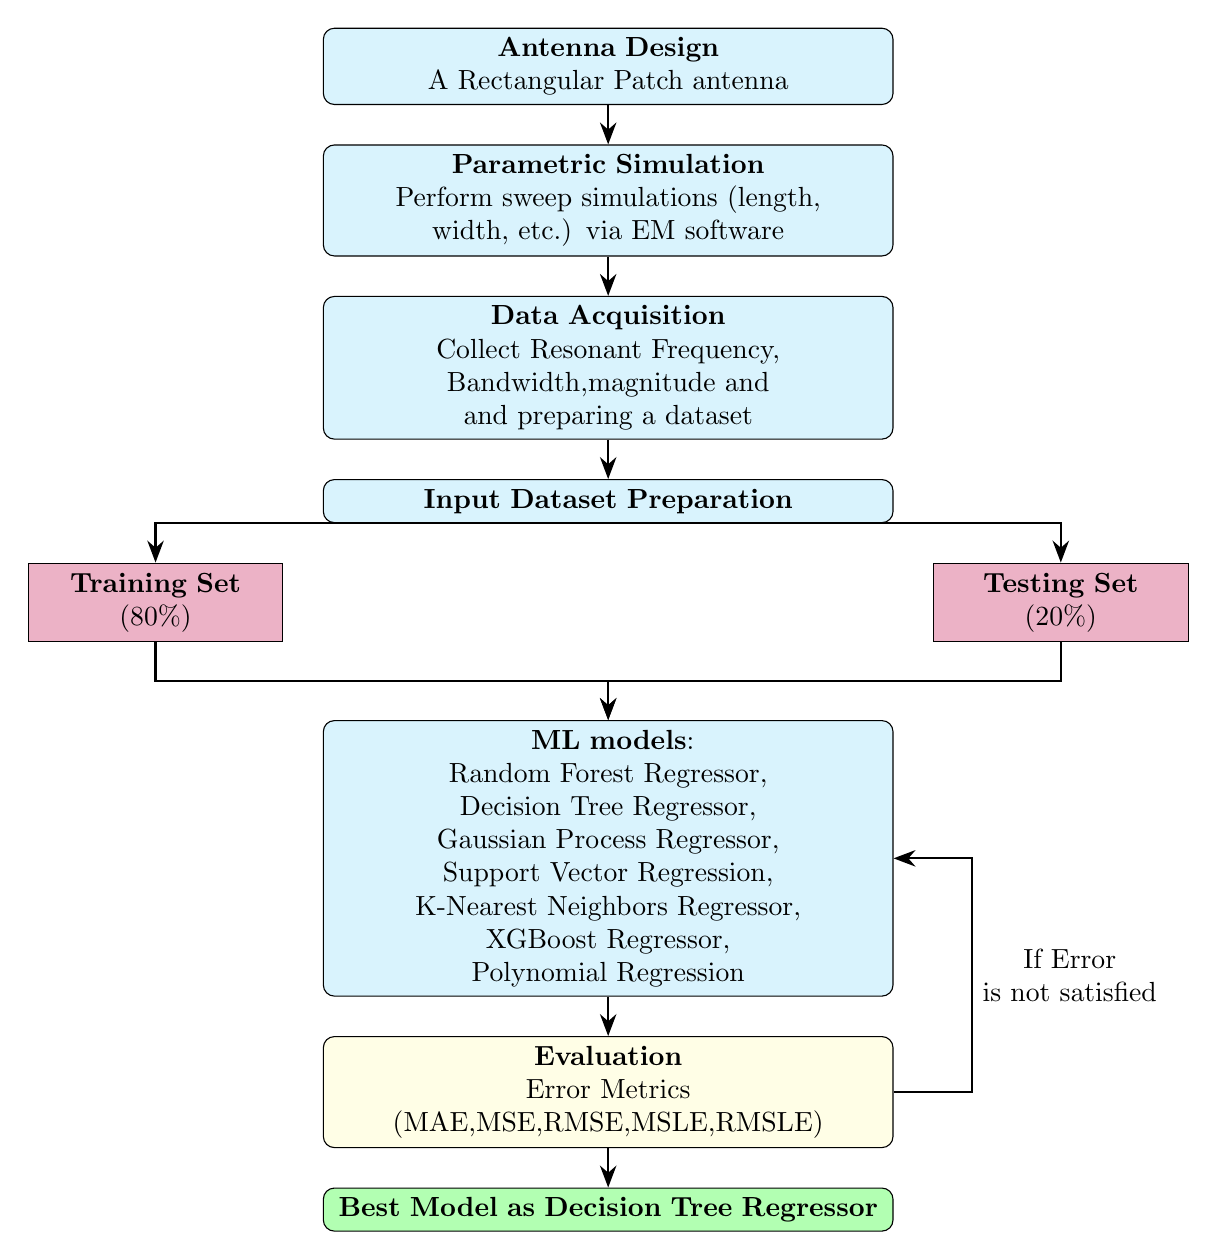
\begin{tikzpicture}[
    node distance=0.5cm,
    block/.style={rectangle, draw, fill=cyan!15, text width=7cm, align=center, rounded corners, minimum height=0.5cm},
    split/.style={rectangle, draw, fill=purple!30, text width=3cm, align=center, minimum height=1cm},
    decision/.style={diamond, draw, fill=yellow!20, text width=2cm, align=center, inner sep=0pt},
    arrow/.style={thick, -{Stealth[scale=1.2]}}
]

% --- Nodes ---
\node (design) [block] {\textbf{Antenna Design}\\A Rectangular Patch antenna};

\node (sim) [block, below=of design] {\textbf{Parametric Simulation}\\Perform sweep simulations (length, width, etc.) via EM software};

\node (data) [block, below=of sim] {\textbf{Data Acquisition}\\Collect Resonant Frequency, Bandwidth,magnitude and and preparing a dataset};

\node (input) [block, below=of data, fill=cyan!15] {\textbf{Input Dataset Preparation}};

% Splitting the data
\node (train) [split, below left=0.5cm and 0.5cm of input] {\textbf{Training Set}\\(80\%)};
\node (test) [split, below right=0.5cm and 0.5cm of input] {\textbf{Testing Set}\\(20\%)};

\node (ml) [block, below=2.5cm of input] {\textbf{
ML models}:\\
Random Forest Regressor,\\
Decision Tree Regressor,\\
Gaussian Process Regressor,\\
Support Vector Regression,\\
K-Nearest Neighbors Regressor,\\
XGBoost Regressor,\\
Polynomial Regression};

\node (eval) [block, below=of ml, fill=yellow!10] {\textbf{Evaluation}\\Error Metrics (MAE,MSE,RMSE,MSLE,RMSLE)};

\node (best) [block, below=of eval, fill=green!30] {\textbf{Best Model as Decision Tree Regressor}};

% --- Arrows ---
\draw [arrow] (design) -- (sim);
\draw [arrow] (sim) -- (data);
\draw [arrow] (data) -- (input);

\draw [arrow] (input.south) -| (train.north);
\draw [arrow] (input.south) -| (test.north);

\draw [arrow] (train.south) |- ([yshift=0.5cm]ml.north) -- (ml.north);
\draw [arrow] (test.south) |- ([yshift=0.5cm]ml.north) -- (ml.north);

\draw [arrow] (ml) -- (eval);
\draw [arrow] (eval) -- (best);

% Feedback loop
\draw [arrow] (eval.east) -- ++(1,0) |- node[pos=0.25, right, align=center] {If Error\\is not satisfied} (ml.east);

\end{tikzpicture}

\end{document}
